\PassOptionsToPackage{unicode=true}{hyperref} % options for packages loaded elsewhere
\PassOptionsToPackage{hyphens}{url}
%
\documentclass[ignorenonframetext,]{beamer}
\setbeamertemplate{caption}[numbered]
\setbeamertemplate{caption label separator}{: }
\setbeamercolor{caption name}{fg=normal text.fg}
\beamertemplatenavigationsymbolsempty
\usepackage{lmodern}
\usepackage{amssymb,amsmath}
\usepackage{ifxetex,ifluatex}
\usepackage{fixltx2e} % provides \textsubscript
\ifnum 0\ifxetex 1\fi\ifluatex 1\fi=0 % if pdftex
  \usepackage[T1]{fontenc}
  \usepackage[utf8]{inputenc}
  \usepackage{textcomp} % provides euro and other symbols
\else % if luatex or xelatex
  \usepackage{unicode-math}
  \defaultfontfeatures{Ligatures=TeX,Scale=MatchLowercase}
\fi
% use upquote if available, for straight quotes in verbatim environments
\IfFileExists{upquote.sty}{\usepackage{upquote}}{}
% use microtype if available
\IfFileExists{microtype.sty}{%
\usepackage[]{microtype}
\UseMicrotypeSet[protrusion]{basicmath} % disable protrusion for tt fonts
}{}
\IfFileExists{parskip.sty}{%
\usepackage{parskip}
}{% else
\setlength{\parindent}{0pt}
\setlength{\parskip}{6pt plus 2pt minus 1pt}
}
\usepackage{hyperref}
\hypersetup{
            pdftitle={Neuroconductor and Imaging Statistics in R},
            pdfauthor={John Muschelli http://johnmuschelli.com/smi\_2018},
            pdfborder={0 0 0},
            breaklinks=true}
\urlstyle{same}  % don't use monospace font for urls
\newif\ifbibliography
\usepackage{graphicx,grffile}
\makeatletter
\def\maxwidth{\ifdim\Gin@nat@width>\linewidth\linewidth\else\Gin@nat@width\fi}
\def\maxheight{\ifdim\Gin@nat@height>\textheight\textheight\else\Gin@nat@height\fi}
\makeatother
% Scale images if necessary, so that they will not overflow the page
% margins by default, and it is still possible to overwrite the defaults
% using explicit options in \includegraphics[width, height, ...]{}
\setkeys{Gin}{width=\maxwidth,height=\maxheight,keepaspectratio}
% Prevent slide breaks in the middle of a paragraph:
\widowpenalties 1 10000
\raggedbottom
\setbeamertemplate{part page}{
\centering
\begin{beamercolorbox}[sep=16pt,center]{part title}
  \usebeamerfont{part title}\insertpart\par
\end{beamercolorbox}
}
\setbeamertemplate{section page}{
\centering
\begin{beamercolorbox}[sep=12pt,center]{part title}
  \usebeamerfont{section title}\insertsection\par
\end{beamercolorbox}
}
\setbeamertemplate{subsection page}{
\centering
\begin{beamercolorbox}[sep=8pt,center]{part title}
  \usebeamerfont{subsection title}\insertsubsection\par
\end{beamercolorbox}
}
\AtBeginPart{
  \frame{\partpage}
}
\AtBeginSection{
  \ifbibliography
  \else
    \frame{\sectionpage}
  \fi
}
\AtBeginSubsection{
  \frame{\subsectionpage}
}
\setlength{\emergencystretch}{3em}  % prevent overfull lines
\providecommand{\tightlist}{%
  \setlength{\itemsep}{0pt}\setlength{\parskip}{0pt}}
\setcounter{secnumdepth}{0}

% set default figure placement to htbp
\makeatletter
\def\fps@figure{htbp}
\makeatother


\title{Neuroconductor and Imaging Statistics in R}
\providecommand{\subtitle}[1]{}
\subtitle{\url{https://github.com/muschellij2/Neuroimaging_in_R}}
\author{John Muschelli \url{http://johnmuschelli.com/smi_2018}}
\date{}
\logo{
\includegraphics{bloomberg.logo.small.horizontal.blue.png}}

\begin{document}
\frame{\titlepage}

\begin{frame}[fragile]

\begin{block}{CRAN Packages 5-10 years ago vs.~today}

\begin{itemize}
\tightlist
\item
  BioC+GitHub \texttt{15258} (\url{https://www.rdocumentation.org/})
\end{itemize}

Script from \url{https://gist.github.com/daroczig/3cf06d6db4be2bbe3368}

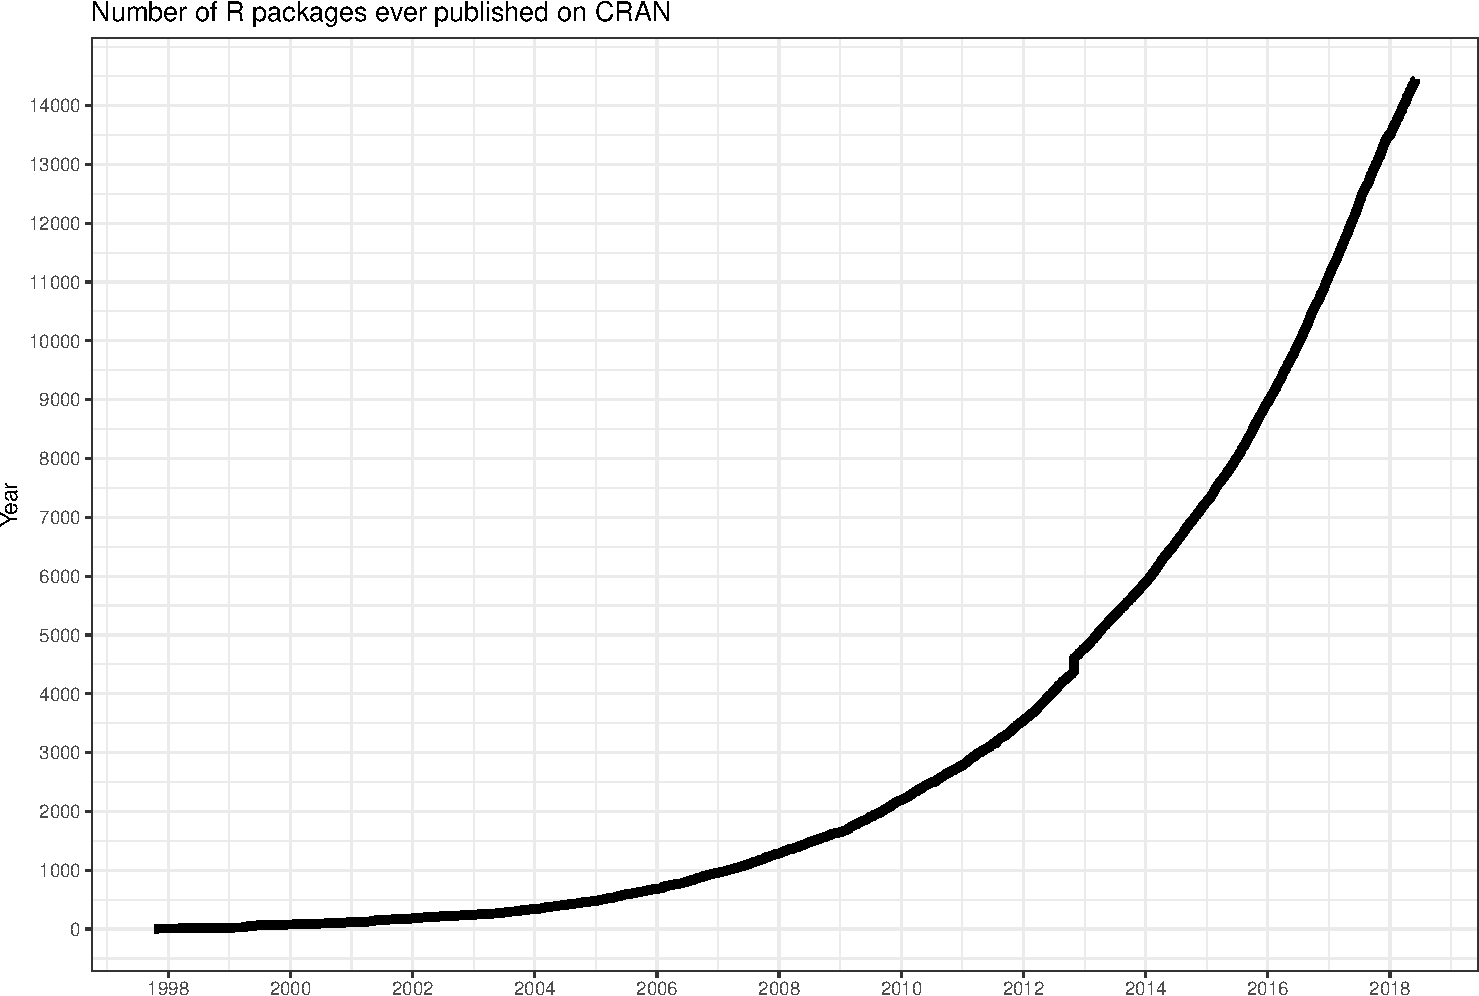
\includegraphics{index_files/figure-beamer/unnamed-chunk-1-1.pdf}

\end{block}

\begin{block}{Imaging in R: 5 years ago}

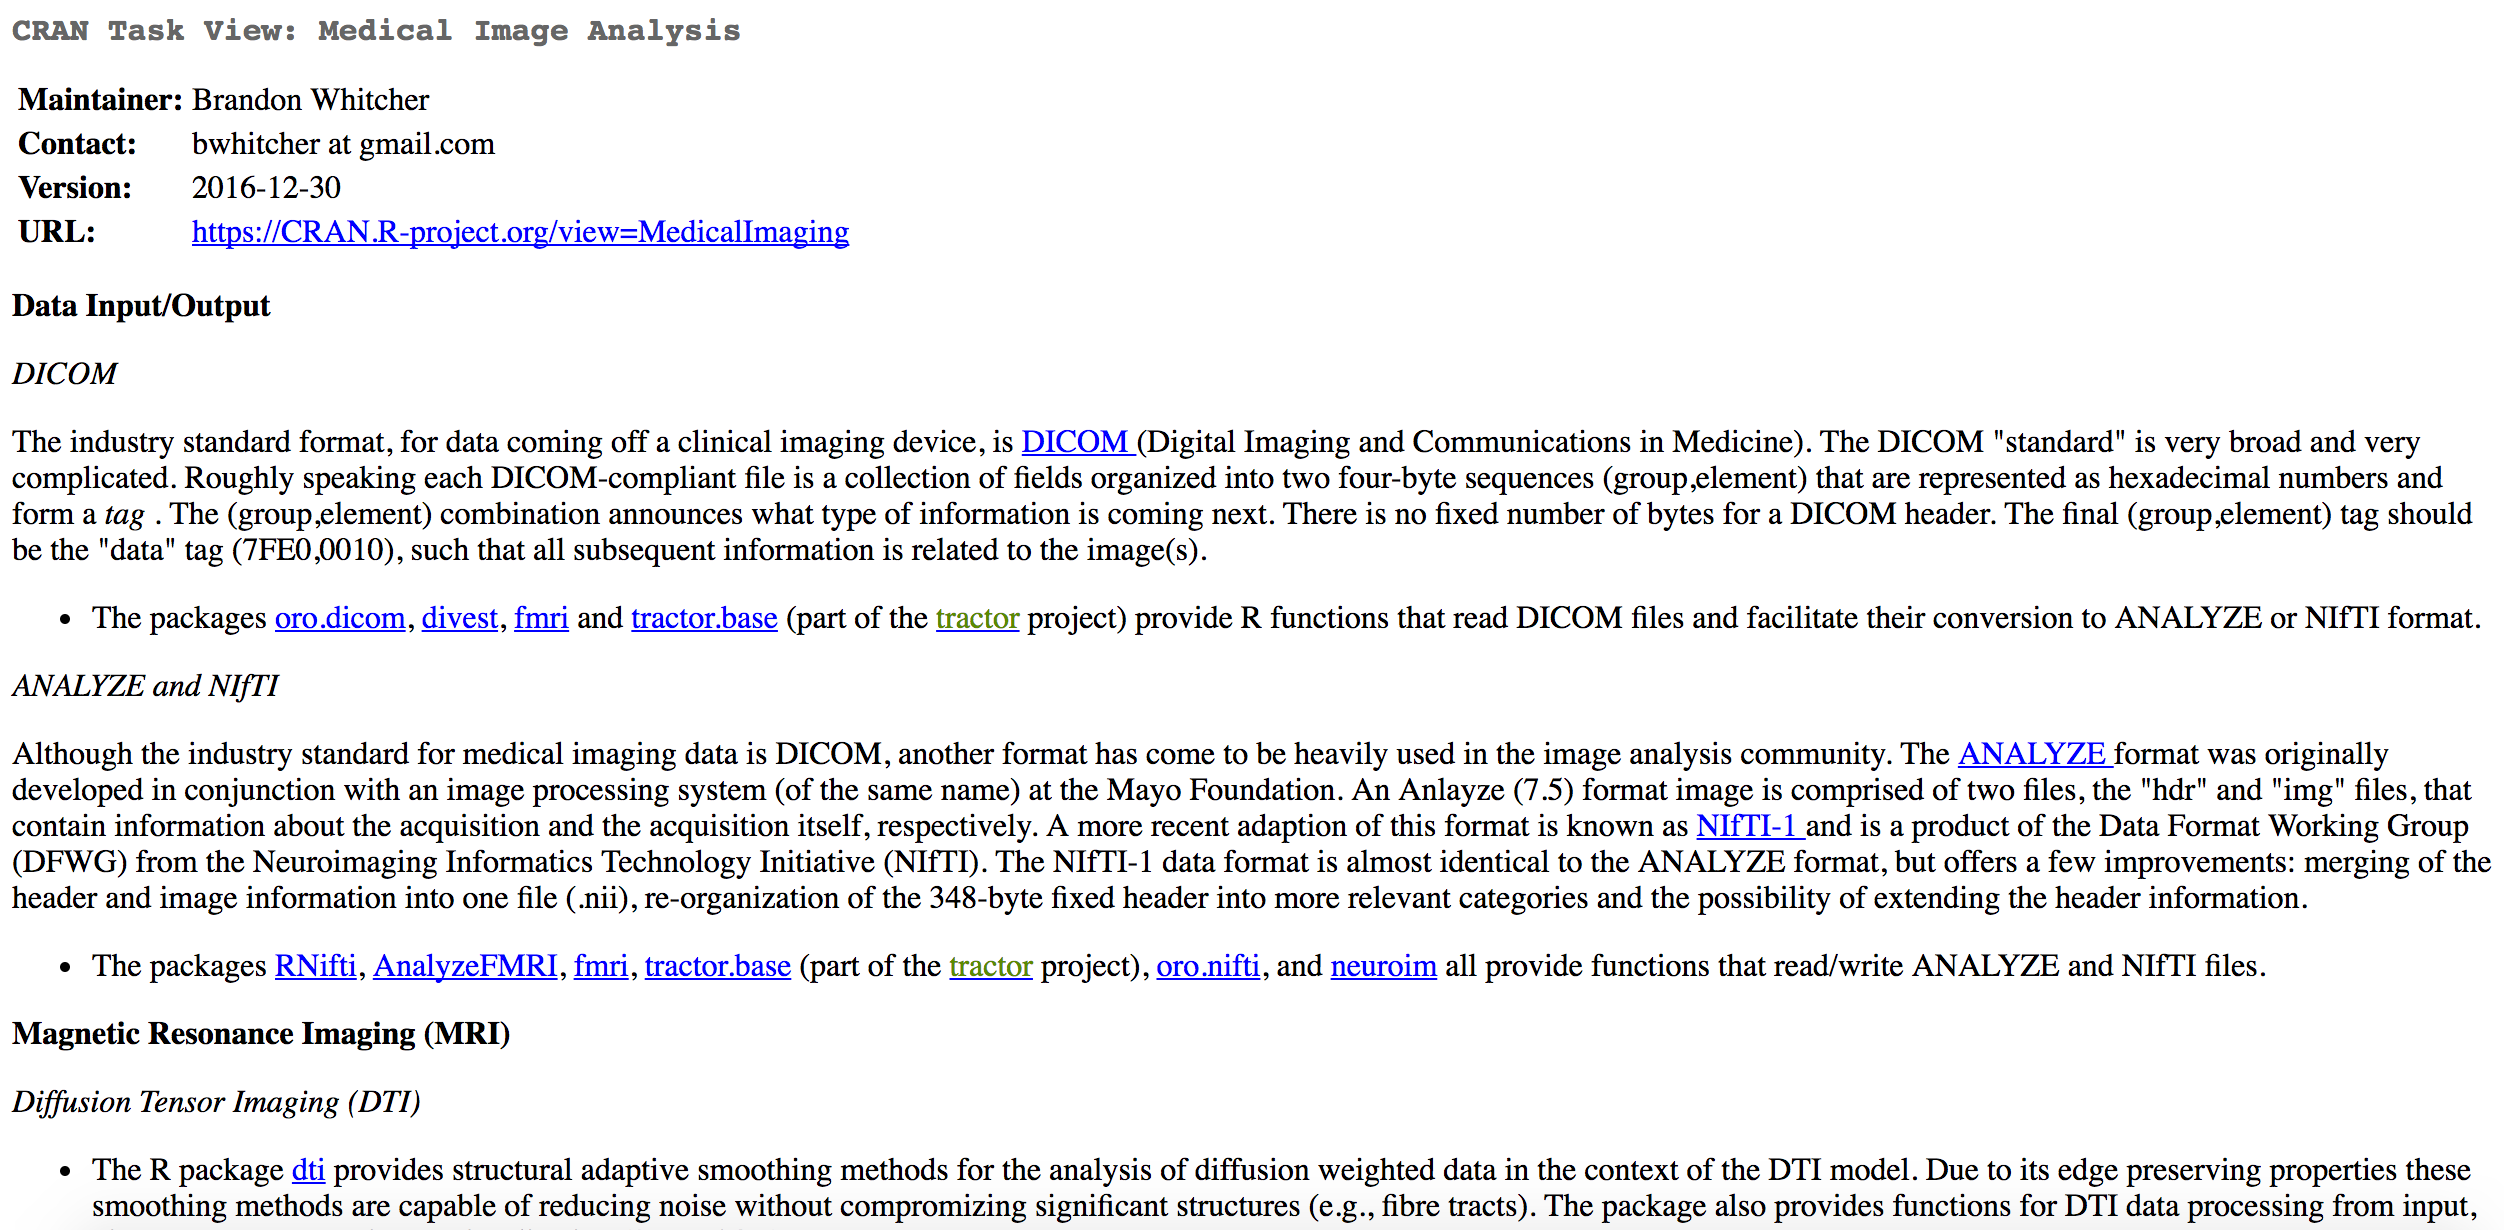
\includegraphics[width=0.95\linewidth]{figure/imaging_task_view}

\end{block}

\end{frame}

\begin{frame}

\hypertarget{left_col2}{}
Workflow: 5 years ago

\begin{itemize}
\tightlist
\item
  bash 
\item
  FSL 
\item
  ANTs 
\item
  MRIcroGL 
\item
  OsiriX 
\item
  SPM 12 
\end{itemize}

\hypertarget{right_col2}{}

\end{frame}

\begin{frame}

\hypertarget{left_col2}{}
Workflow: 5 years ago

Multiple pieces of software used

\begin{itemize}
\tightlist
\item
  all different syntax
\end{itemize}

\hypertarget{right_col2}{}

\end{frame}

\begin{frame}{R: Programming and Interface Language}
\protect\hypertarget{r-programming-and-interface-language}{}

\end{frame}

\begin{frame}[fragile]

\hypertarget{left_col2}{}
Workflow: Now

\begin{itemize}
\tightlist
\item
  all R code

  \begin{itemize}
  \tightlist
  \item
    interface/pipeline tool
  \item
    “native” R code
  \end{itemize}
\end{itemize}

Complete pipeline

\begin{itemize}
\tightlist
\item
  preprocessing and analysis
\end{itemize}

\hypertarget{right_col2}{}

\begin{block}{Imaging in R: Now}

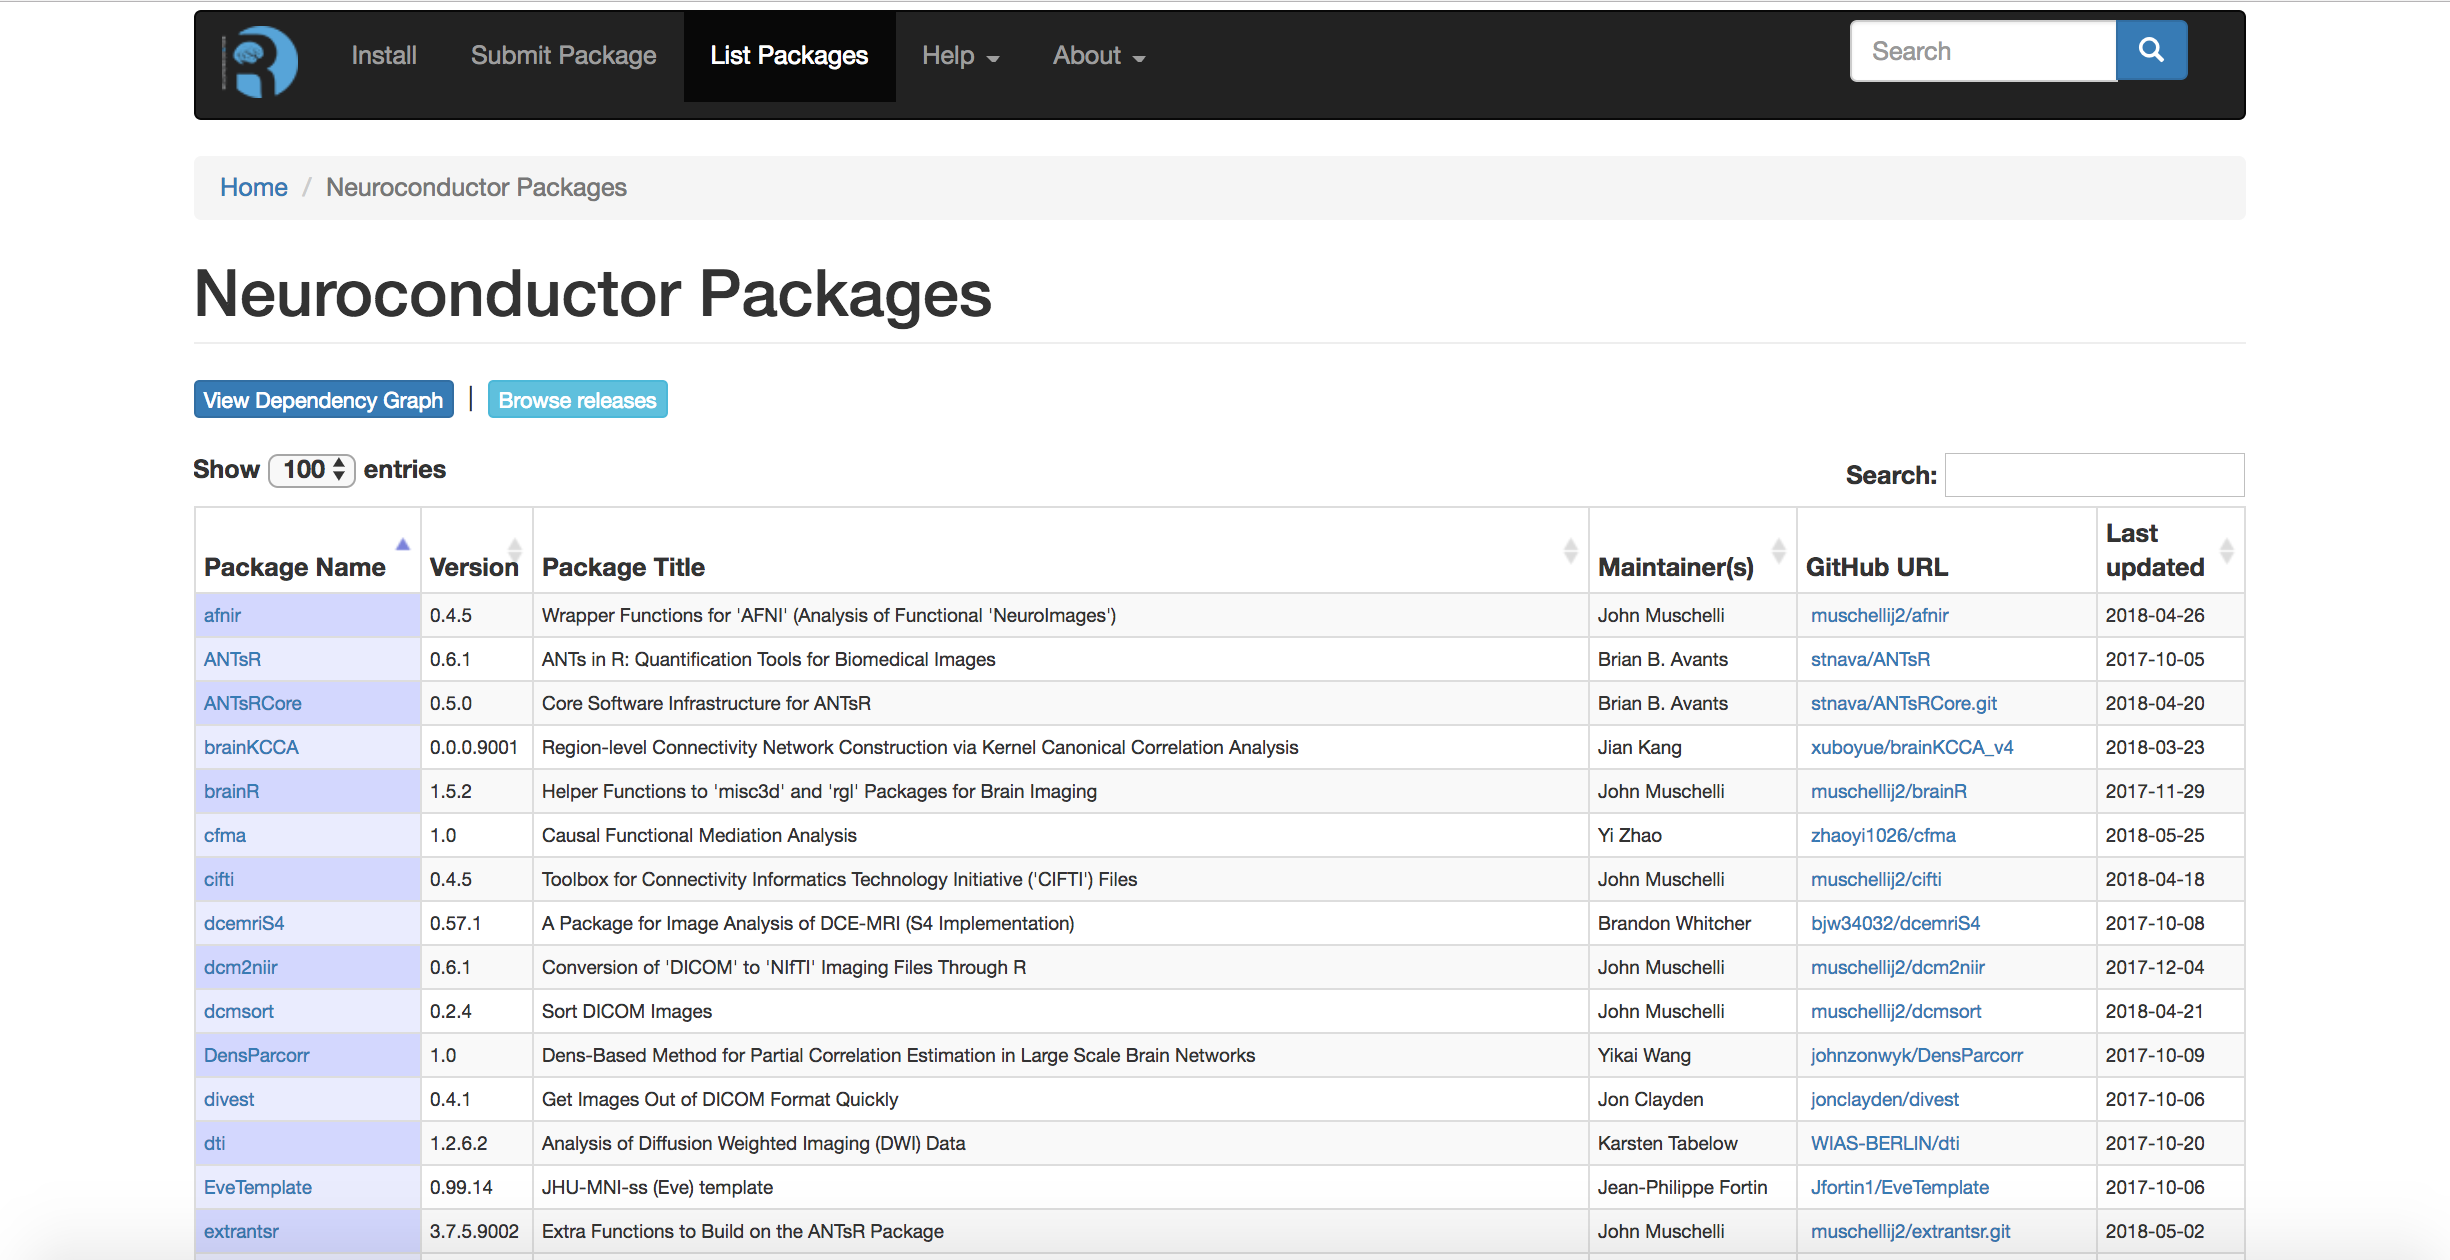
\includegraphics[width=0.95\linewidth]{figure/neuroc}

\end{block}

\begin{block}{Weaknesses of Imaging in R}

\hypertarget{left_col}{}
\begin{itemize}
\tightlist
\item
  Speed, but \texttt{Rcpp}, not always ported to \texttt{Rcpp}

  \begin{itemize}
  \tightlist
  \item
    A lot of work to inferface with large libraries
  \end{itemize}
\item
  Memory issues
\item
  MATLAB is more popular and has GUIs
\item
  System Dependencies are not handled well in packages
\end{itemize}

\hypertarget{right_col}{}
\includegraphics[width=1\linewidth]{figure/need_for_speed}

\url{https://giphy.com/gifs/top-gun-need-for-speed-i-feel-the-26AHLNr8en8J3ovOo}

\begin{itemize}
\tightlist
\item
  e.g. (fsl, FSL, install FSL at
  \url{https://fsl.fmrib.ox.ac.uk/fsl/fslwiki/FslInstallation})
\end{itemize}

\end{block}

\begin{block}{Strengths of Imaging in R}

\hypertarget{left_col}{}
\begin{itemize}
\tightlist
\item
  Free
\item
  Large/strong R community
\item
  RStudio
\item
  Validated statistical models
\item
  Package development system
\item
  Neuroconductor
\item
  Shiny
\end{itemize}

\hypertarget{right_col}{}

\includegraphics[width=1\linewidth]{figure/always_use_r}

\url{https://imgflip.com/i/2blglk}

\end{block}

\begin{block}{Threats of Imaging in R}

\begin{itemize}
\tightlist
\item
  Not much different than Python

  \begin{itemize}
  \tightlist
  \item
    scikit-learn/ Nipype
  \end{itemize}
\item
  Neural Networks
\item
  BME have tools for advanced statistical analysis
\item
  \textbf{Study design is not as valued in imaging (neuro)}

  \begin{itemize}
  \tightlist
  \item
    one stronghold of statisticians
  \end{itemize}
\item
  Credit/Incentives for software
\end{itemize}

\end{block}

\begin{block}{Opportunities of Imaging in R}

\hypertarget{left_col}{}
\begin{itemize}
\tightlist
\item
  Neural Networks: Keras and Tensorflow
\item
  Genomic analyses are very similar

  \begin{itemize}
  \tightlist
  \item
    use Bioconductor tools in a new way
  \end{itemize}
\end{itemize}

\hypertarget{right_col}{}

\includegraphics[width=1\linewidth]{figure/bioc_tools}

\url{https://imgflip.com/i/2bmb3c}

\end{block}

\begin{block}{Threats to}

\end{block}

\begin{block}{Opportunities: CONSORT diagrams}

\url{https://imgflip.com/i/2bltgh}

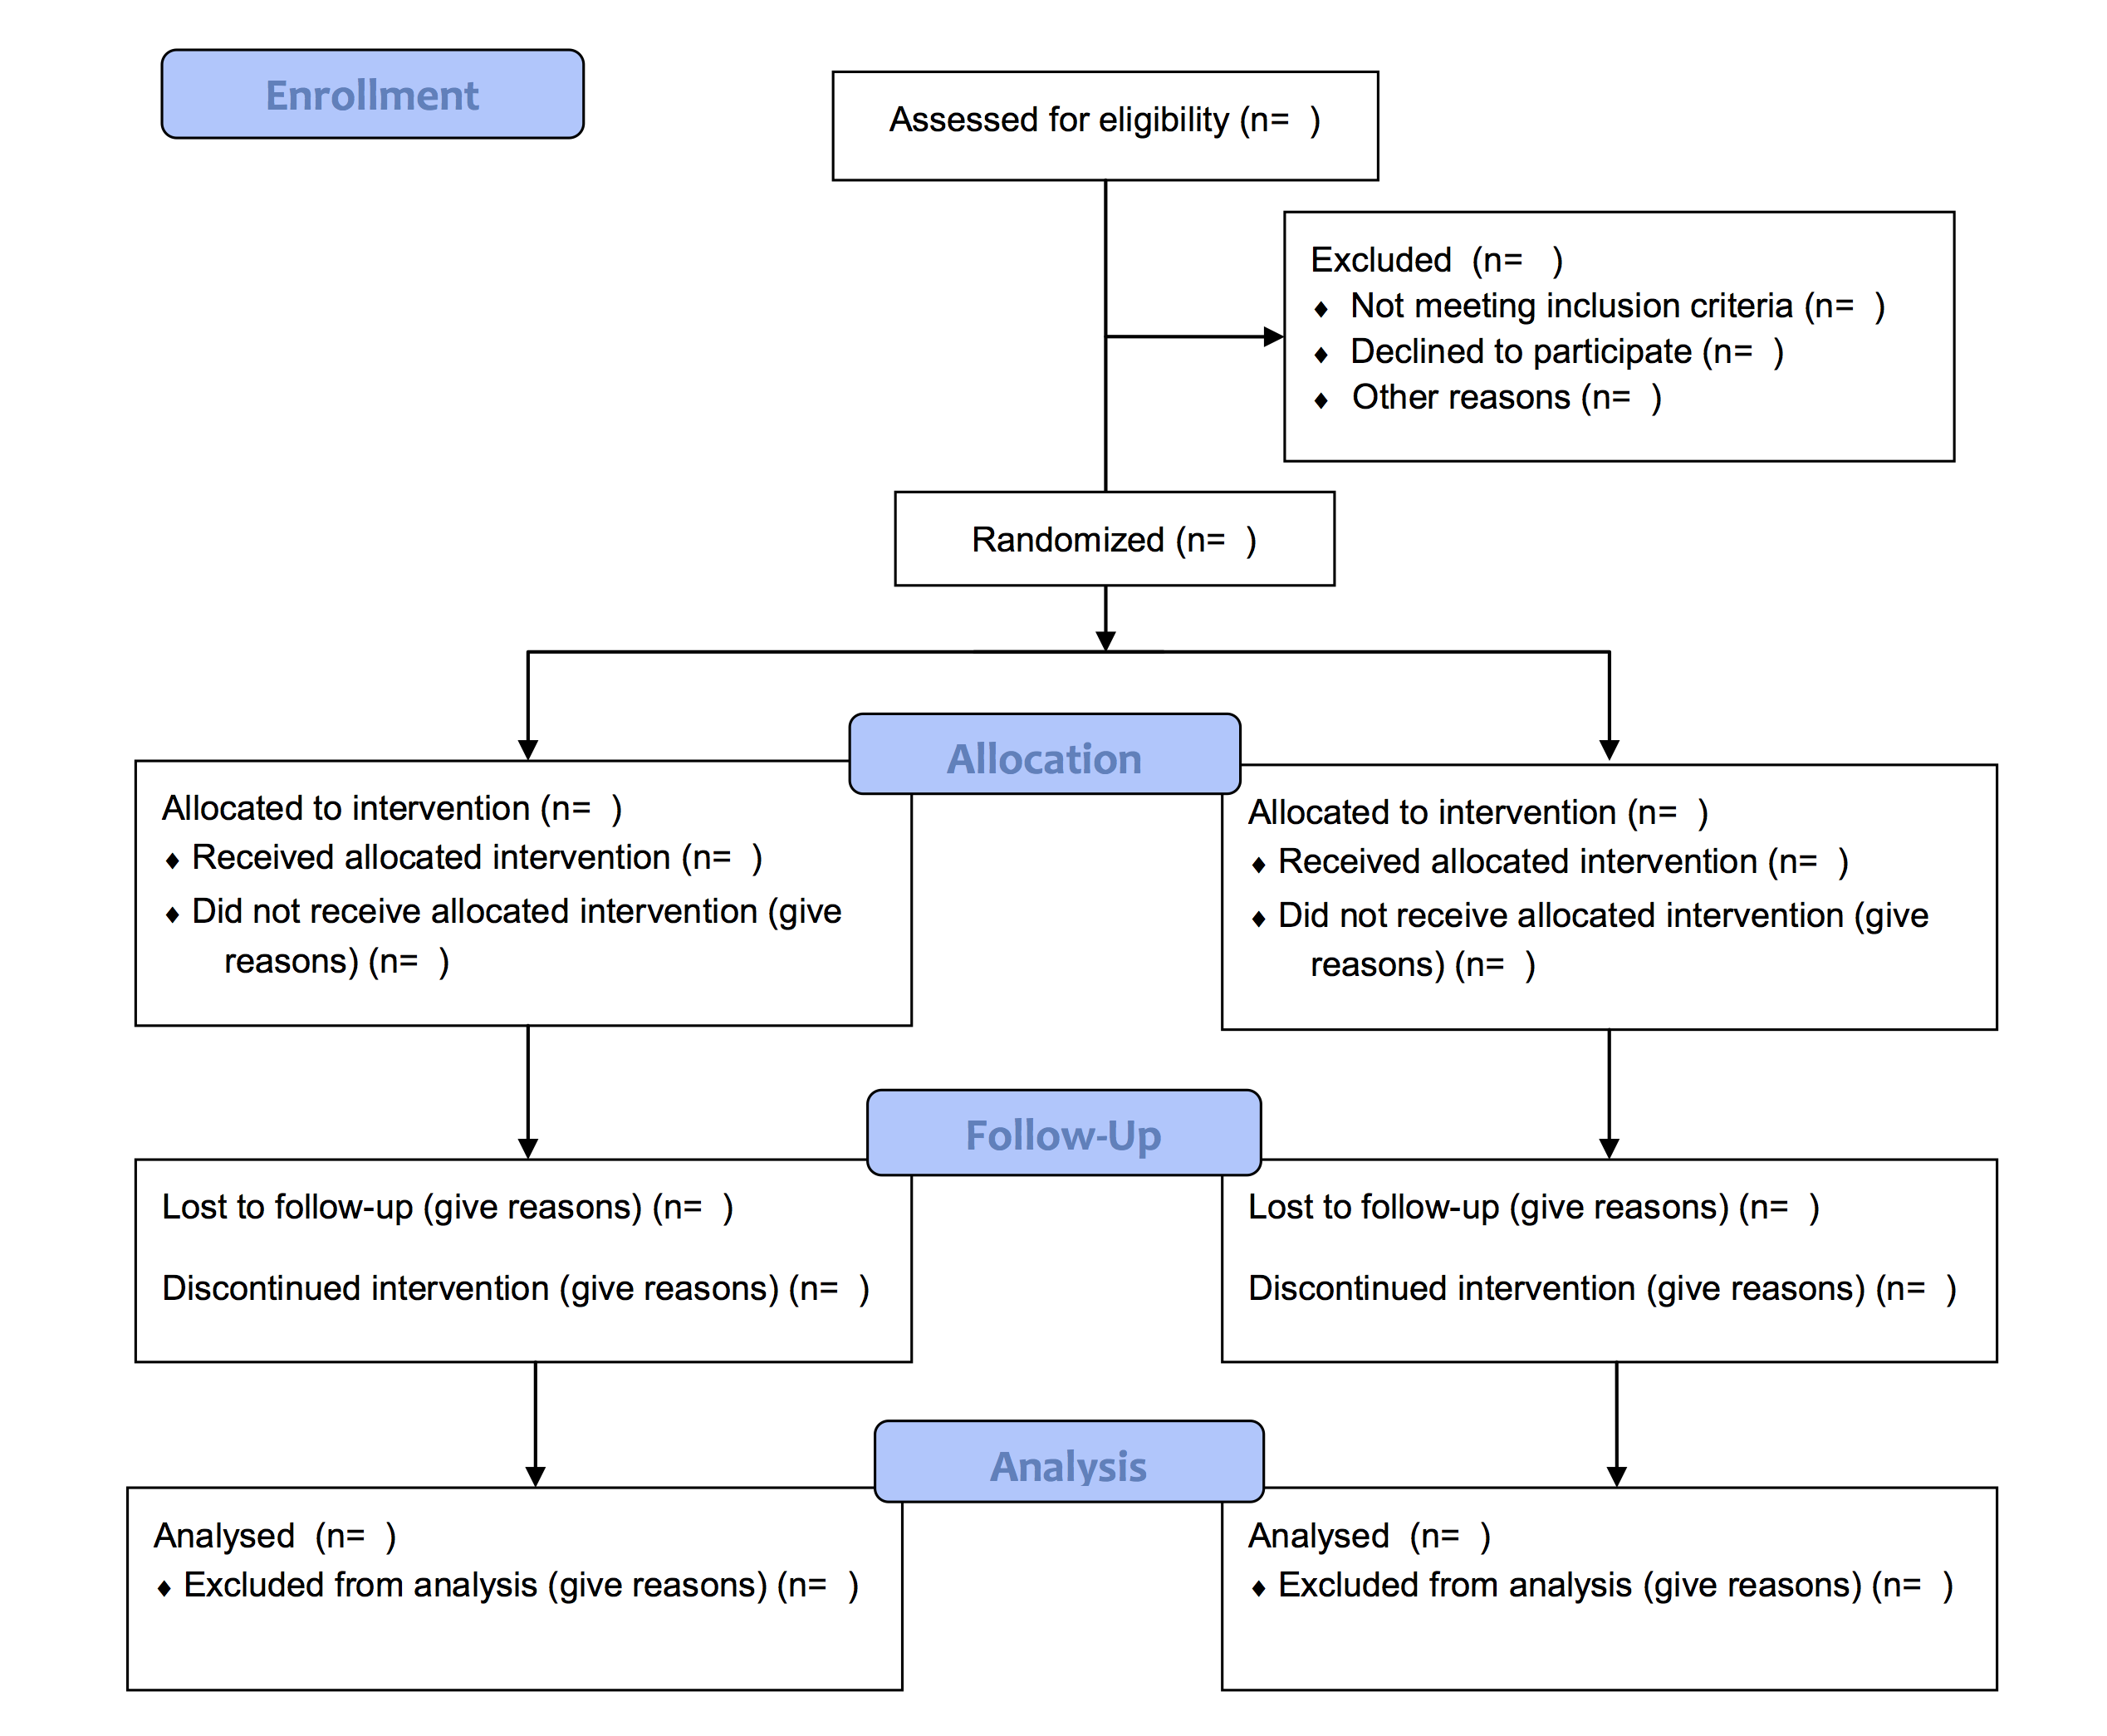
\includegraphics[width=0.9\linewidth]{figure/consort}

\end{block}

\begin{block}{Opportunities: Moving from Linear Models}

\begin{itemize}
\tightlist
\item
  Task fMRI: compare baseline to 1+ conditions
\item
  Smoothed to account for neighborhood
\item
  Run LM on time-series voxelwise with AR-type correlation with
  HRF-convolved design matrix (\(X\)) + motion/other factors (\(Z\))
\end{itemize}

\[
Y_{iv} = X_{i} \beta_{iv} + Z_{i}\theta_{iv} + \varepsilon_{iv} \\
\varepsilon_{iv} \sim N(0, \Sigma_{iv}) \\
\Sigma_{iv} \sim \text{AR}
\]

\(Z_{i}\) can be different for each \(i\) (scrubbing), but usually
isn’t.

\end{block}

\begin{block}{Opportunities of Stats in Imaging}

\begin{itemize}
\tightlist
\item
  Get \(β_i\) map in MNI space
\item
  Run t-test, random effects analysis (hard to find sometimes), or
  permutation test
\item
  Perform multiple comparisons correction (maybe with spatial compoent)
\end{itemize}

\end{block}

\begin{block}{Opportunities of Stats in Imaging}

\hypertarget{left_col}{}
\begin{itemize}
\tightlist
\item
  What if the motion had a non-linear effect?

  \begin{itemize}
  \tightlist
  \item
    currently: use derivatives and squared effects
  \item
    why not GAMs? (speed)\texttt{voxel} package
  \end{itemize}
\item
  fully Bayes (spatial) hard because of data size (maybe empirical)
\end{itemize}

\hypertarget{right_col}{}

\includegraphics[width=1.2\linewidth]{figure/nonlinear}

\url{https://imgflip.com/i/2bltw2}

\end{block}

\end{frame}

\begin{frame}[fragile]

\leavevmode\hypertarget{left_col}{}%
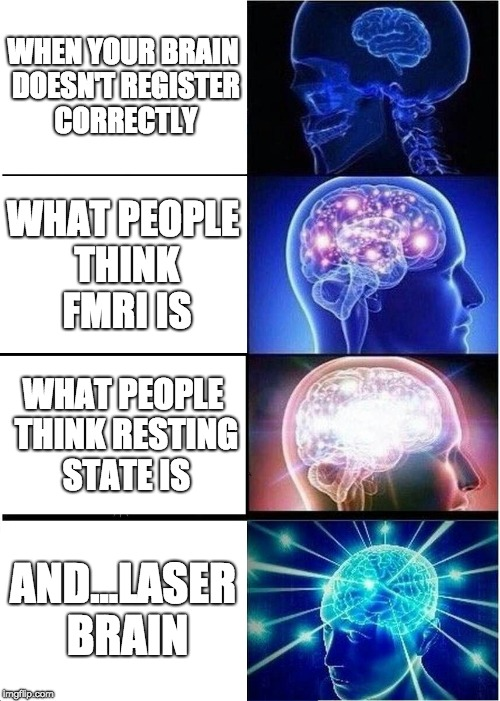
\includegraphics[width=0.7\linewidth]{figure/laser_brain}

Opportunities of Stats in Imaging: Laser Brain

\url{https://imgflip.com/i/2blg14}

\begin{block}{Opportunities of Stats in Imaging}

\hypertarget{left_col}{}
\begin{itemize}
\tightlist
\item
  \textbf{Multi-site/multi-scanner data from consortium}

  \begin{itemize}
  \tightlist
  \item
    batch effects abound\\
  \end{itemize}
\end{itemize}

\hypertarget{right_col}{}

\includegraphics[width=1.2\linewidth]{figure/batch_effect}

\url{https://imgflip.com/i/2blid6}

\end{block}

\begin{block}{Opportunities: Data}

\end{block}

\begin{block}{What we need: tutorials}

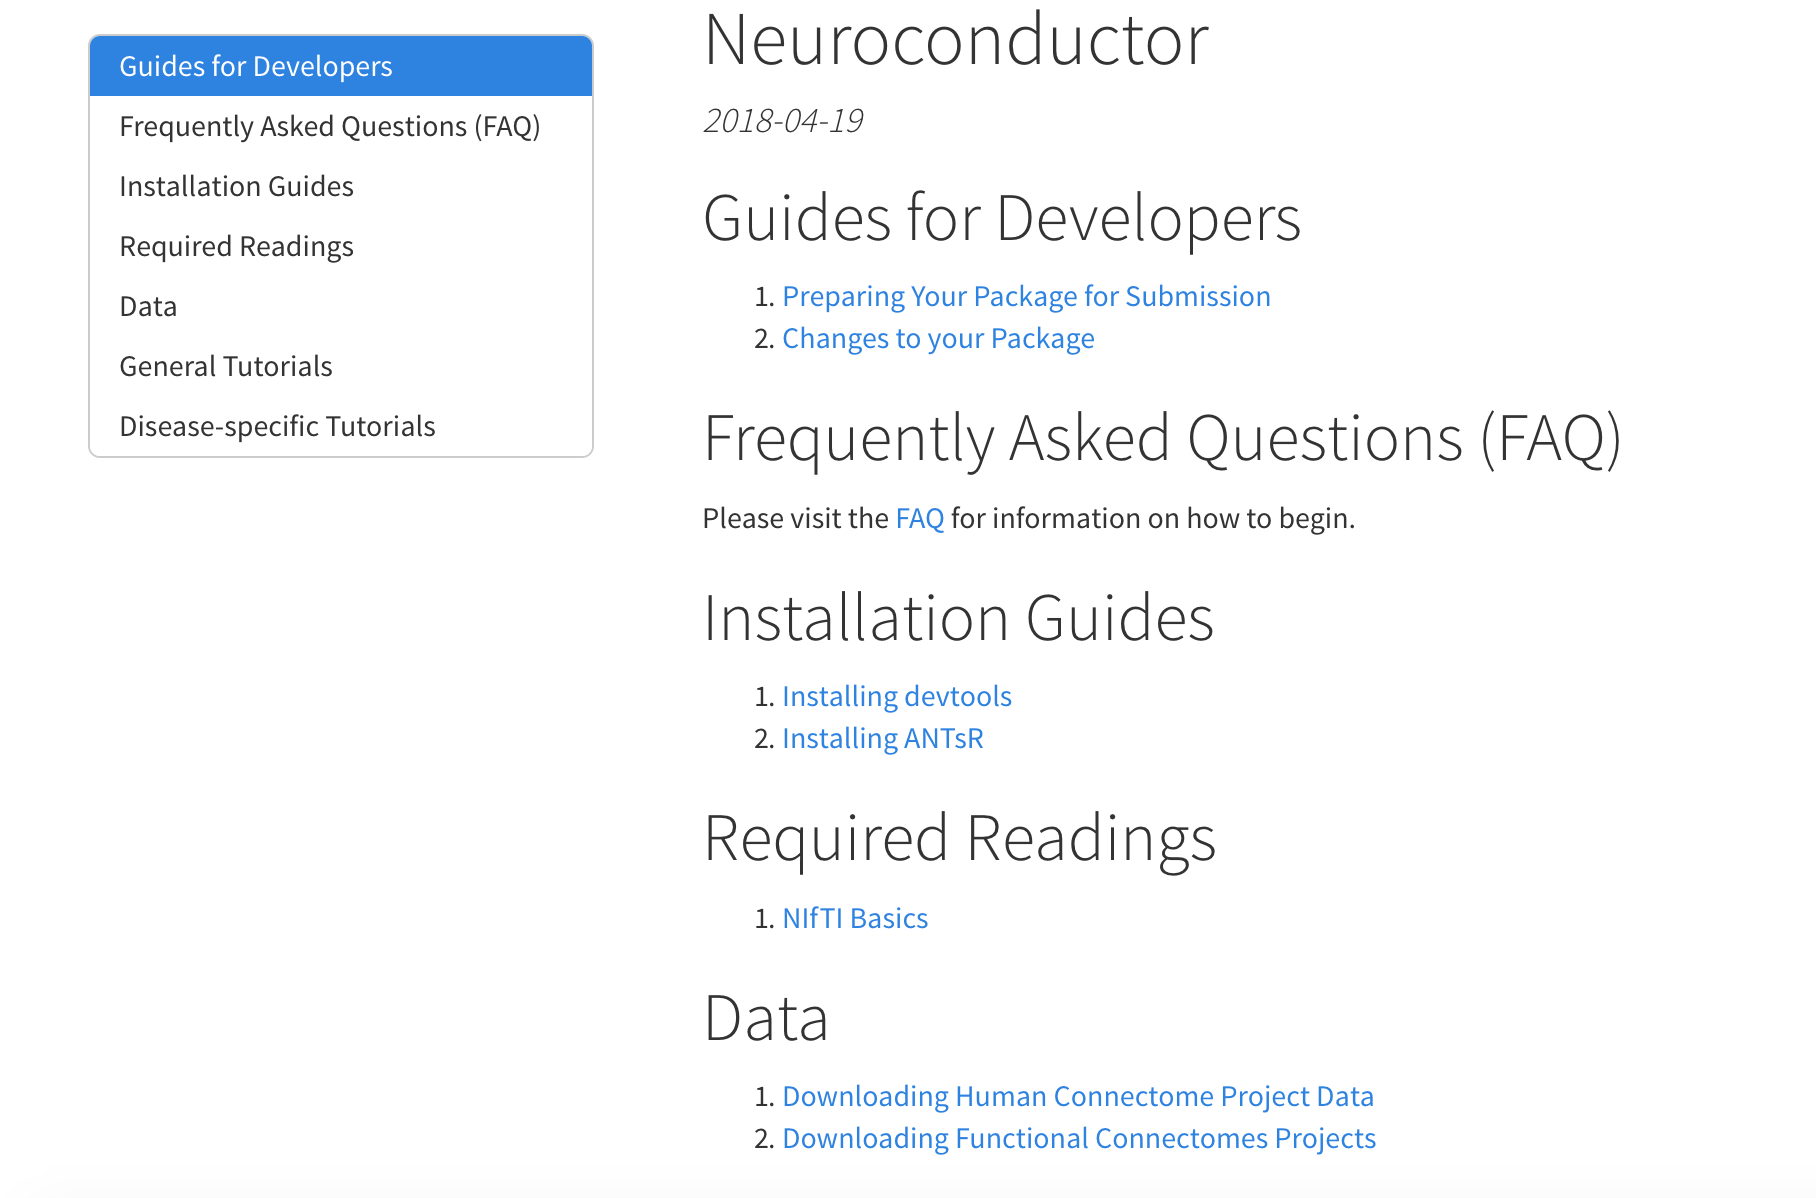
\includegraphics[width=0.95\linewidth]{figure/tutorials}

\end{block}

\begin{block}{What we really need: tutorials on fMRI}

\begin{itemize}
\tightlist
\item
  \texttt{preprocessfMRI} from ANTsR
\item
  \texttt{spm12r} -
  \url{https://neuroconductor.org/neuroc-help-fmri-analysis-spm12r}
\item
  \texttt{fslr} -
  \url{https://neuroconductor.org/neuroc-help-fmri-analysis-fslr}
\end{itemize}

\end{block}

\end{frame}

\begin{frame}{What we need: Shiny GUIs}
\protect\hypertarget{what-we-need-shiny-guis}{}

\begin{block}{(Maybe) What we need: challenges}

\url{https://grand-challenge.org/all_challenges/}

\includegraphics[width=0.95\linewidth]{figure/grandchallenges}

\end{block}

\begin{block}{“Pre”-processing is Important}


\includegraphics[width=1\linewidth]{figure/know_processing}

\url{https://imgflip.com/i/2blh8f}

\end{block}

\begin{block}{“Pre”-processing is Hard}


\includegraphics[width=1\linewidth]{figure/know_processing}

\url{https://imgflip.com/i/2blh8f}


\includegraphics[width=0.75\linewidth]{figure/choose_smoothing}

\url{https://imgflip.com/i/2blhsc}

\end{block}

\end{frame}

\begin{frame}[fragile]{Package Showcase}
\protect\hypertarget{package-showcase}{}

\begin{block}{Data}

\begin{itemize}
\tightlist
\item
  \texttt{EveTemplate}/\texttt{MNITemplate} - templates
\item
  \texttt{kirby21} series
\item
  \texttt{sri24} - SRI24 MRI Atlas
\item
  \texttt{malf.templates} - templates for label fusion
\item
  \texttt{neurohcp} - download data from HCP/INDI
\item
  \texttt{nitrcbot} - download data from NITRC
\item
  \texttt{neurovault} - download data from \url{https://neurovault.org/}
\end{itemize}

\end{block}

\begin{block}{General Imaging Tools}

\begin{itemize}
\tightlist
\item
  \texttt{EBImage} - image processing and analysis
\item
  \texttt{magick} - Bindings to ImageMagick
\item
  OpenCV:
  \href{https://github.com/swarm-lab/ROpenCVLite}{\texttt{swarm-lab/ROpenCVLite}}
  or
  \href{https://github.com/ropenscilabs/opencv}{\texttt{ropenscilabs/opencv}}
\item
  \texttt{ANTsR} - a large imaging suite (mainly neuro)
\end{itemize}

\end{block}

\begin{block}{Starting from Raw Data/DICOM}

\begin{itemize}
\tightlist
\item
  \texttt{oro.dicom} - read/write DICOM data
\item
  \texttt{dcm2niir} - uses \texttt{dcm2niix} from Chris Rorden
\item
  \texttt{divest} - \texttt{Rcpp} wrapped \texttt{dcm2niix}
\item
  \texttt{dcmtk} - interface package for DCMTK
\item
  \texttt{matlabr} - could use \texttt{dicomread} MATLAB code and
  excecute through R
\end{itemize}

\end{block}

\begin{block}{Interactive Visualization using papayaWidget}

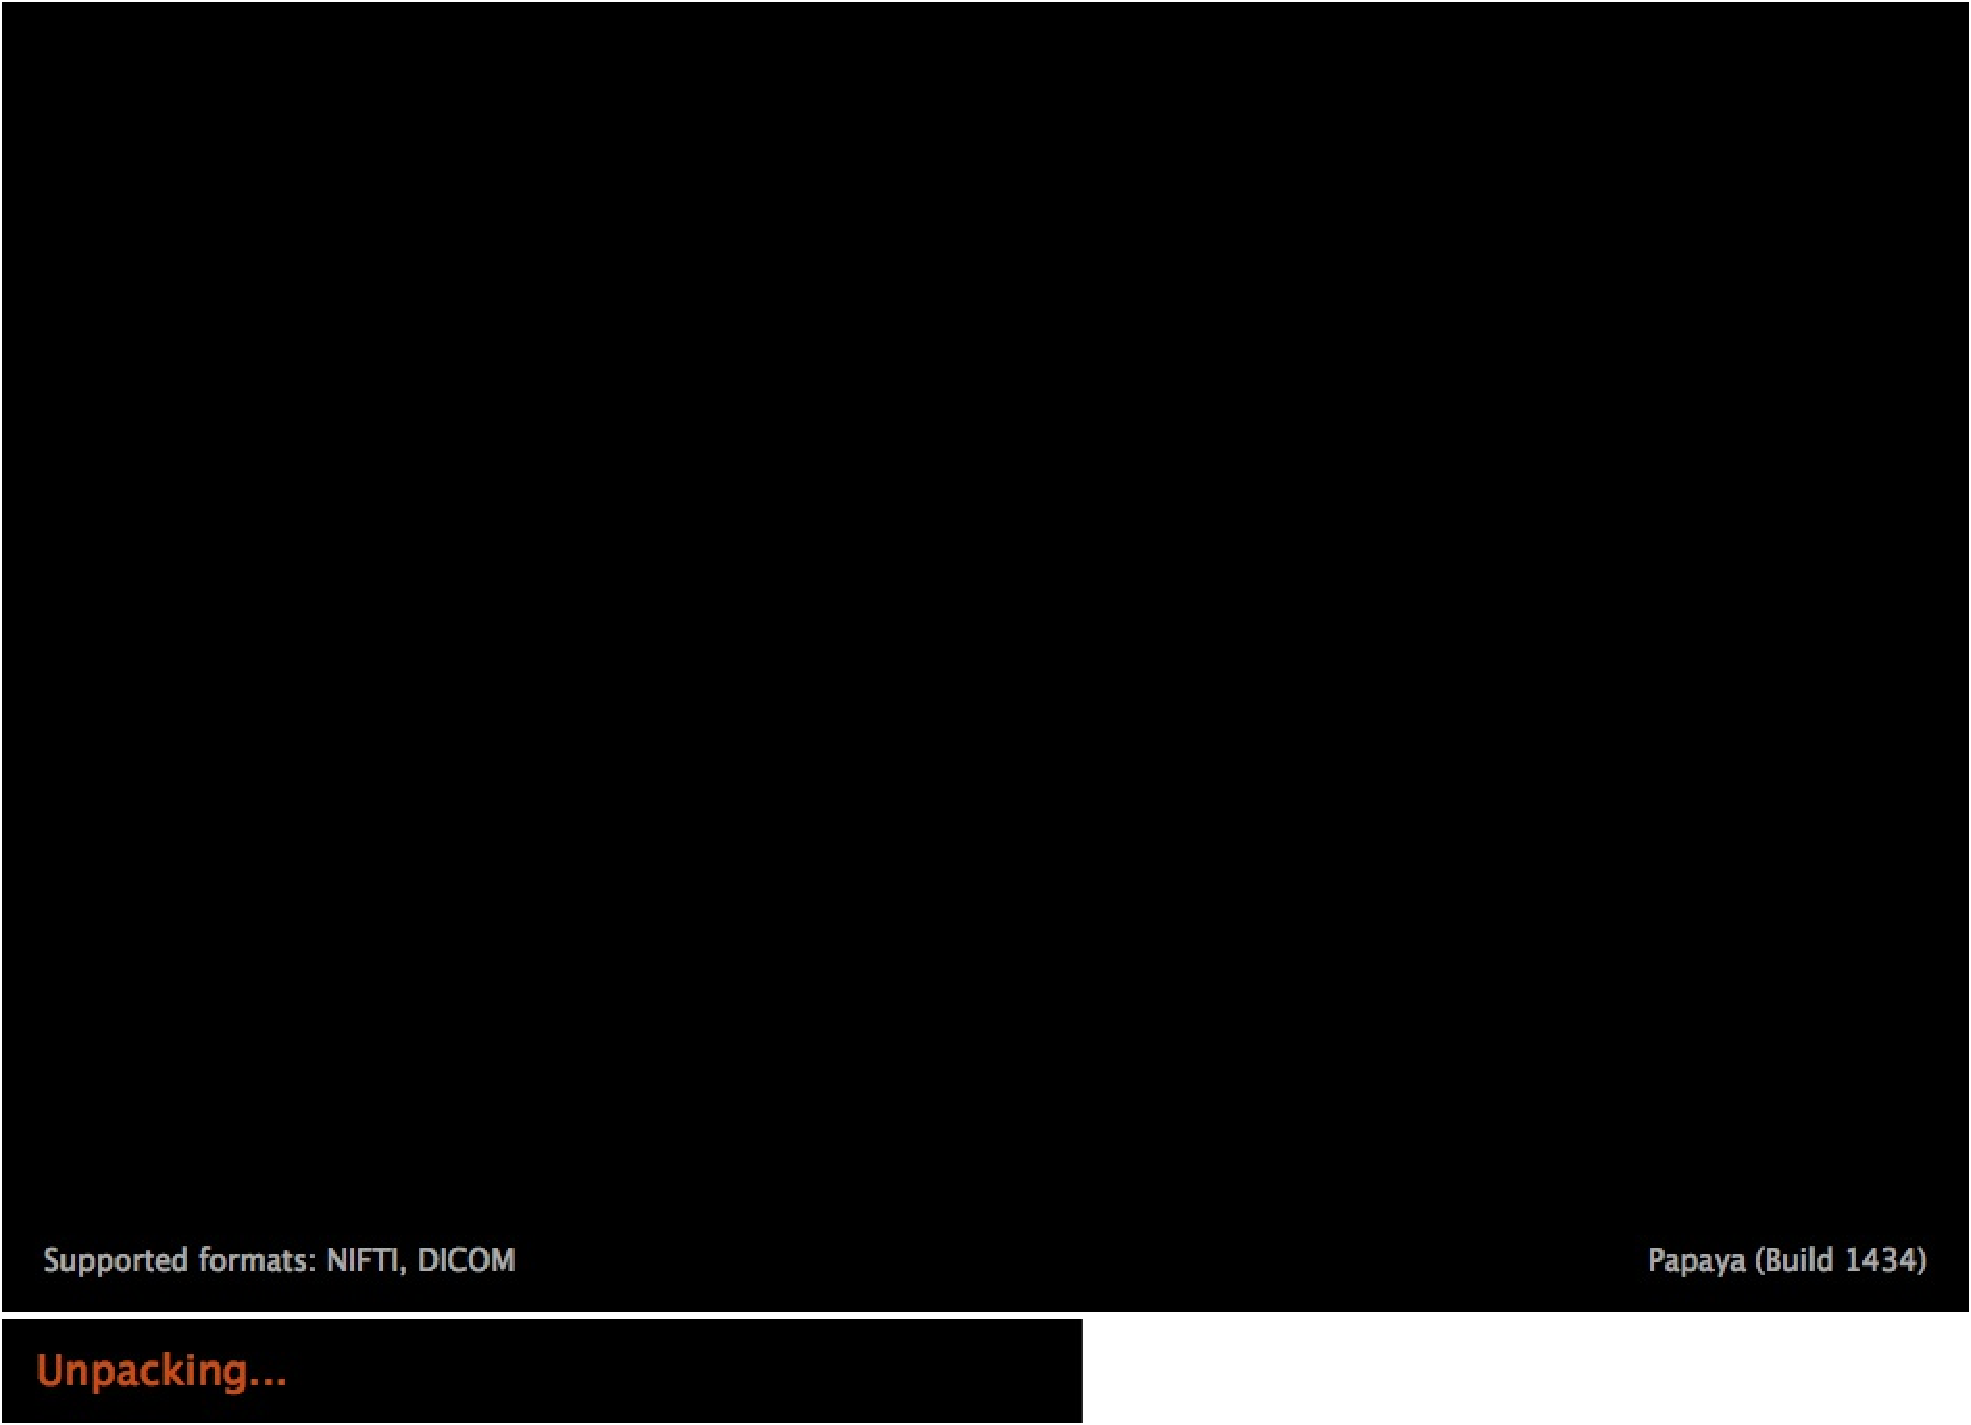
\includegraphics{index_files/figure-beamer/unnamed-chunk-16-1.pdf}

\end{block}

\begin{block}{\texttt{ggneuro} visualization: \texttt{ggplot2} object}

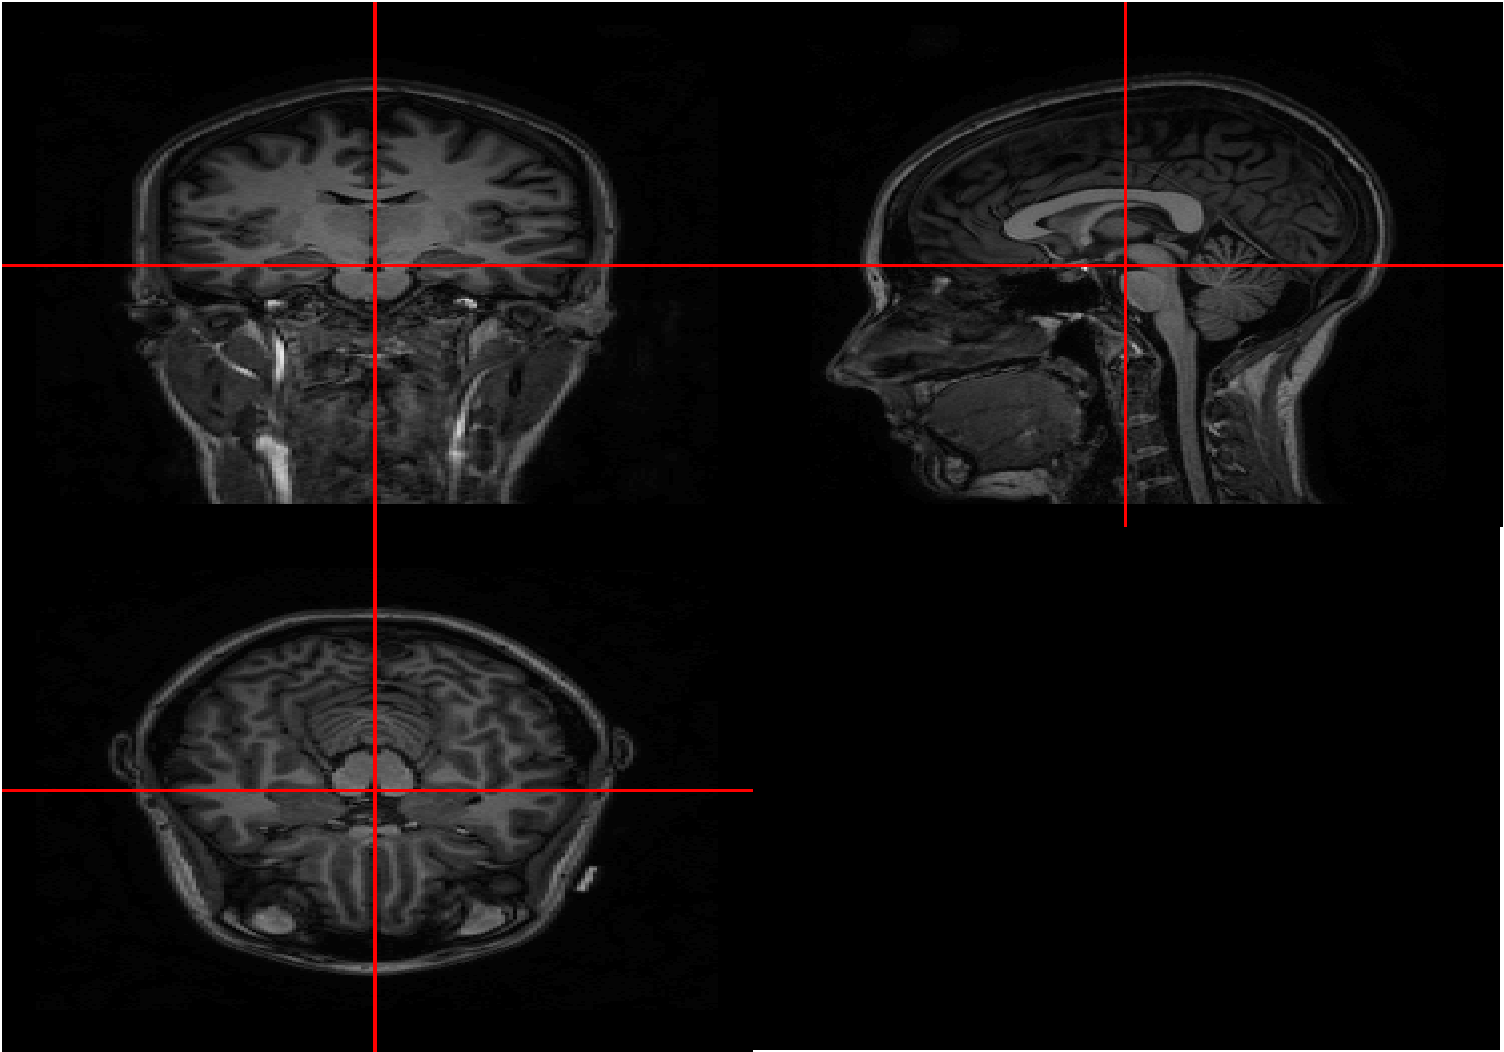
\includegraphics{index_files/figure-beamer/unnamed-chunk-17-1.pdf}

\end{block}

\begin{block}{Intensity Normalization}

\begin{itemize}
\tightlist
\item
  \texttt{whitestripe} - WhiteStripe (Shinohara et al. 2014)
\item
  Quantile transform \texttt{quantile\_img} (in \texttt{neurobase})
\item
  Whole brain z-scoring: \texttt{zscore\_img} in \texttt{neurobase}
\item
  \texttt{RAVEL} - Fortin et al. (2016)
\item
  Histogram matching (in \texttt{RAVEL})
\item
  General standardization methods
\end{itemize}

\end{block}

\begin{block}{MS Lesion Segmentation}

\begin{itemize}
\tightlist
\item
  \texttt{sublime} - E. Sweeney et al. (2013)
\item
  \texttt{oasis} - Sweeney et al. (2013)
\item
  \texttt{mimosa} - Valcarcel et al. (2018)
\item
  \texttt{smri.process} - my package on sMRI processing
\end{itemize}

\end{block}

\begin{block}{Step 1: Image Processing: Workflow}

The N4 (Tustison et al. 2010) EM-style model assumed is: \[
\log(x(v)) = \log(u(v)) + \log( f(v) )
\]

\begin{itemize}
\tightlist
\item
  \(x\): given image
\item
  \(u\): uncorrupted image
\item
  \(f\): bias field
\item
  \(v\): location in the image
\end{itemize}

\end{block}

\begin{block}{Image Processing: MALF}

\leavevmode\hypertarget{left_col}{}%
Figure from MASS paper (Doshi et al. 2013):

\hypertarget{right_col}{}
\begin{itemize}
\tightlist
\item
  Register templates to an image using the T1 for that subject
\item
  Apply transformation to the label/mask
\item
  Average each voxel over all templates

  \begin{itemize}
  \tightlist
  \item
    there are “smarter” (e.g.~weighted) ways
  \end{itemize}
\end{itemize}

\end{block}

\begin{block}{Step 2: Create Predictors for each Sequence}

\leavevmode\hypertarget{left_col}{}%

\hypertarget{right_col}{}
\begin{itemize}
\tightlist
\item
  Predictors created with intensity-normalized data

  \begin{itemize}
  \tightlist
  \item
    Quantile images, smoothers, local moments
  \end{itemize}
\item
  Tissue class probability with local moments: MALF and FAST (Zhang,
  Brady, and Smith 2001)
\item
  Z-score to a population template
\end{itemize}

\end{block}

\begin{block}{A package to do all this: \texttt{smri.process}}

\begin{itemize}
\tightlist
\item
  GitHub package (\texttt{muschellij2/smri.process})
\end{itemize}

\end{block}

\begin{block}{Publishing software}

\begin{itemize}
\tightlist
\item
  R Journal - see \texttt{rticles::rjournal\_article()} (only accept if
  in CRAN)
\item
  F1000 - \url{https://f1000research.com/collections/Neuroconductor}
\item
  JOSS - \url{https://joss.theoj.org/}
\item
  JSS - see \texttt{rticles::jss\_article()}
\item
  \texttt{cranlogs} track downloads
\item
  neuroconductor API tracks downloads
\end{itemize}

\end{block}

\begin{block}{Tracking downloads}

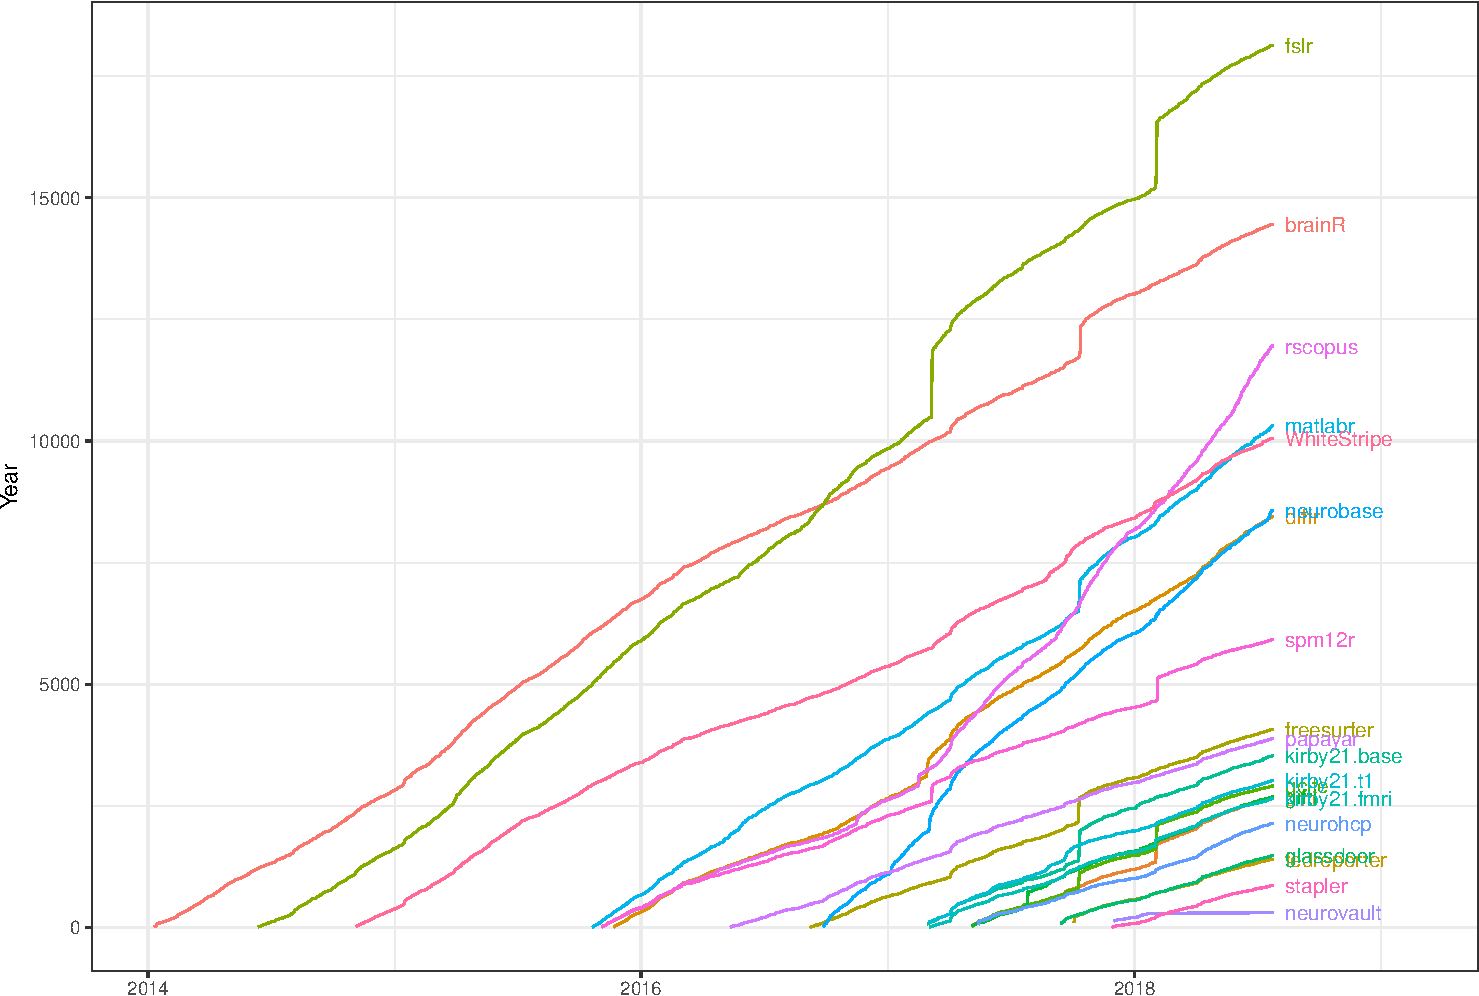
\includegraphics{index_files/figure-beamer/unnamed-chunk-18-1.pdf}

\end{block}

\begin{block}{Conclusions}

\begin{itemize}
\tightlist
\item
  Many methods are being developed for processing neuroimaging in R
\item
  Analysis tools exist but need adaptation
\item
  Develop more standardization like BioConductor

  \begin{itemize}
  \tightlist
  \item
    standard data structures
  \end{itemize}
\item
  GitHub and Neuroconductor
\end{itemize}

\end{block}

\end{frame}

\begin{frame}{Where else can statisicians lead?}
\protect\hypertarget{where-else-can-statisicians-lead}{}

\end{frame}

\begin{frame}[fragile]{Do we need spatial results? If not, why register
to the template?}
\protect\hypertarget{do-we-need-spatial-results-if-not-why-register-to-the-template}{}

\begin{block}{Registration}

ANTsR/extrantsr

\begin{itemize}
\tightlist
\item
  \texttt{antsRegistration} - rigid/affine/non-linear diffeomorphic
\item
  \texttt{extrantsr::registration} - wraps antsRegistration to use
  \texttt{nifti} objects
\end{itemize}

fslr

\begin{itemize}
\tightlist
\item
  \texttt{flirt} - linear/affine registration
\item
  \texttt{fnirt} - non-linear registration (need affine first)
\item
  \texttt{fnirt\_with\_affine} - wraps above 2
\end{itemize}

\end{block}

\begin{block}{Bibliography}

\hypertarget{refs}{}
\leavevmode\hypertarget{ref-mass}{}%
Doshi, Jimit, Guray Erus, Yangming Ou, Bilwaj Gaonkar, and Christos
Davatzikos. 2013. “Multi-Atlas Skull-Stripping.” \emph{Academic
Radiology} 20 (12). Elsevier:1566–76.

\leavevmode\hypertarget{ref-ravel}{}%
Fortin, Jean-Philippe, Elizabeth M Sweeney, John Muschelli, Ciprian M
Crainiceanu, Russell T Shinohara, Alzheimer’s Disease Neuroimaging
Initiative, and others. 2016. “Removing Inter-Subject Technical
Variability in Magnetic Resonance Imaging Studies.” \emph{NeuroImage}
132. Elsevier:198–212.

\leavevmode\hypertarget{ref-shinohara_statistical_2014}{}%
Shinohara, Russell T., Elizabeth M. Sweeney, Jeff Goldsmith, Navid
Shiee, Farrah J. Mateen, Peter A. Calabresi, Samson Jarso, Dzung L.
Pham, Daniel S. Reich, and Ciprian M. Crainiceanu. 2014. “Statistical
Normalization Techniques for Magnetic Resonance Imaging.”
\emph{NeuroImage: Clinical} 6:9–19.
\url{https://doi.org/10.1016/j.nicl.2014.08.008}.

\leavevmode\hypertarget{ref-oasis}{}%
Sweeney, Elizabeth M, Russell T Shinohara, Navid Shiee, Farrah J Mateen,
Avni A Chudgar, Jennifer L Cuzzocreo, Peter A Calabresi, Dzung L Pham,
Daniel S Reich, and Ciprian M Crainiceanu. 2013. “OASIS Is Automated
Statistical Inference for Segmentation, with Applications to Multiple
Sclerosis Lesion Segmentation in MRI.” \emph{NeuroImage: Clinical} 2.
Elsevier:402–13.

\leavevmode\hypertarget{ref-sublime}{}%
Sweeney, EM, RT Shinohara, CD Shea, DS Reich, and CM Crainiceanu. 2013.
“Automatic Lesion Incidence Estimation and Detection in Multiple
Sclerosis Using Multisequence Longitudinal Mri.” \emph{American Journal
of Neuroradiology} 34 (1). Am Soc Neuroradiology:68–73.

\leavevmode\hypertarget{ref-tustison_n4itk_2010}{}%
Tustison, Nicholas J., Brian B. Avants, Philip A. Cook, Yuanjie Zheng,
Alexander Egan, Paul A. Yushkevich, and James C. Gee. 2010. “N4ITK:
Improved N3 Bias Correction.” \emph{IEEE Transactions on Medical
Imaging} 29 (6):1310–20. \url{https://doi.org/10.1109/TMI.2010.2046908}.

\leavevmode\hypertarget{ref-mimosa}{}%
Valcarcel, Alessandra M, Kristin A Linn, Simon N Vandekar, Theodore D
Satterthwaite, John Muschelli, Peter A Calabresi, Dzung L Pham, Melissa
Lynne Martin, and Russell T Shinohara. 2018. “MIMoSA: An Automated
Method for Intermodal Segmentation Analysis of Multiple Sclerosis Brain
Lesions.” \emph{Journal of Neuroimaging}. Wiley Online Library.

\leavevmode\hypertarget{ref-fast}{}%
Zhang, Yongyue, Michael Brady, and Stephen Smith. 2001. “Segmentation of
Brain MR Images Through a Hidden Markov Random Field Model and the
Expectation-Maximization Algorithm.” \emph{Medical Imaging, IEEE
Transactions on} 20 (1):45–57.
\url{http://ieeexplore.ieee.org/xpls/abs_all.jsp?arnumber=906424}.

\end{block}

\end{frame}

\end{document}
